\let\textcircled=\pgftextcircled
\chapter{Theory}
\label{chap:theory}

\initial{T}his is the theory chapter.

%=======
\begin{easylist}[itemize]
\ListProperties(Style*=-- , FinalMark={)}, Margin=0.5cm)
& Give an overview of the fundamental forces and particles.
& Discuss the Standard Model in detail, emphasising certain aspects as they relate to dark matter and the Higgs field (and boson).
& Briefly recap dark matter, referencing descriptions in introduction.
& Discuss the theory behind combined Higgs to inv.: only \acrshort{sm} process in which Higgs decays invisibly is $\PH \rightarrow \PZ\PZ \rightarrow 4\nu$ with branching ratio of 0.1\,\%~\cite{Heinemeyer:1559921}, whilst the current observed experimental limit is 19\,\% from CMS~\cite{Sirunyan:2018owy} and 26\,\% from \acrshort{atlas}~\cite{Aaboud:2019rtt}. If new, invisible particles couple to Higgs, branching ratio will be enhanced. Constraining \BR can also exclude some dark matter models.
& Discuss the theory behind the semi-visible jets analysis (main sources from Refs.~\cite{Cohen:2015toa,Cohen:2017pzm}): strongly interacting dark sector in Hidden Valley scenario with a portal to the visible sector. Mentioning dark quarks \Pqdark, dark confinement scale \lamDark, dark hadronisation and decay, running coupling \aDark, etc.
& Explain some of the phenomenological/experimental event characteristics that overlap with both analyses, i.e., what a jet is, and maybe energy sums like \ptmiss, \HT, \htmiss, etc.
\end{easylist}


\section{The Standard Model}
\label{sec:standardmodel}


\section{Limitations of the Standard Model}
\label{sec:sm_limitations}


\section{Dark matter}
\label{sec:dark_matter}

\subsection{Measuring the branching ratio for the invisible decays of the Higgs boson}
\label{subsec:theory_higgs_to_inv}

\subsection{Searches for semi-visible jets}
\label{subsec:theory_svj}

\begin{figure}[htbp]
\centering
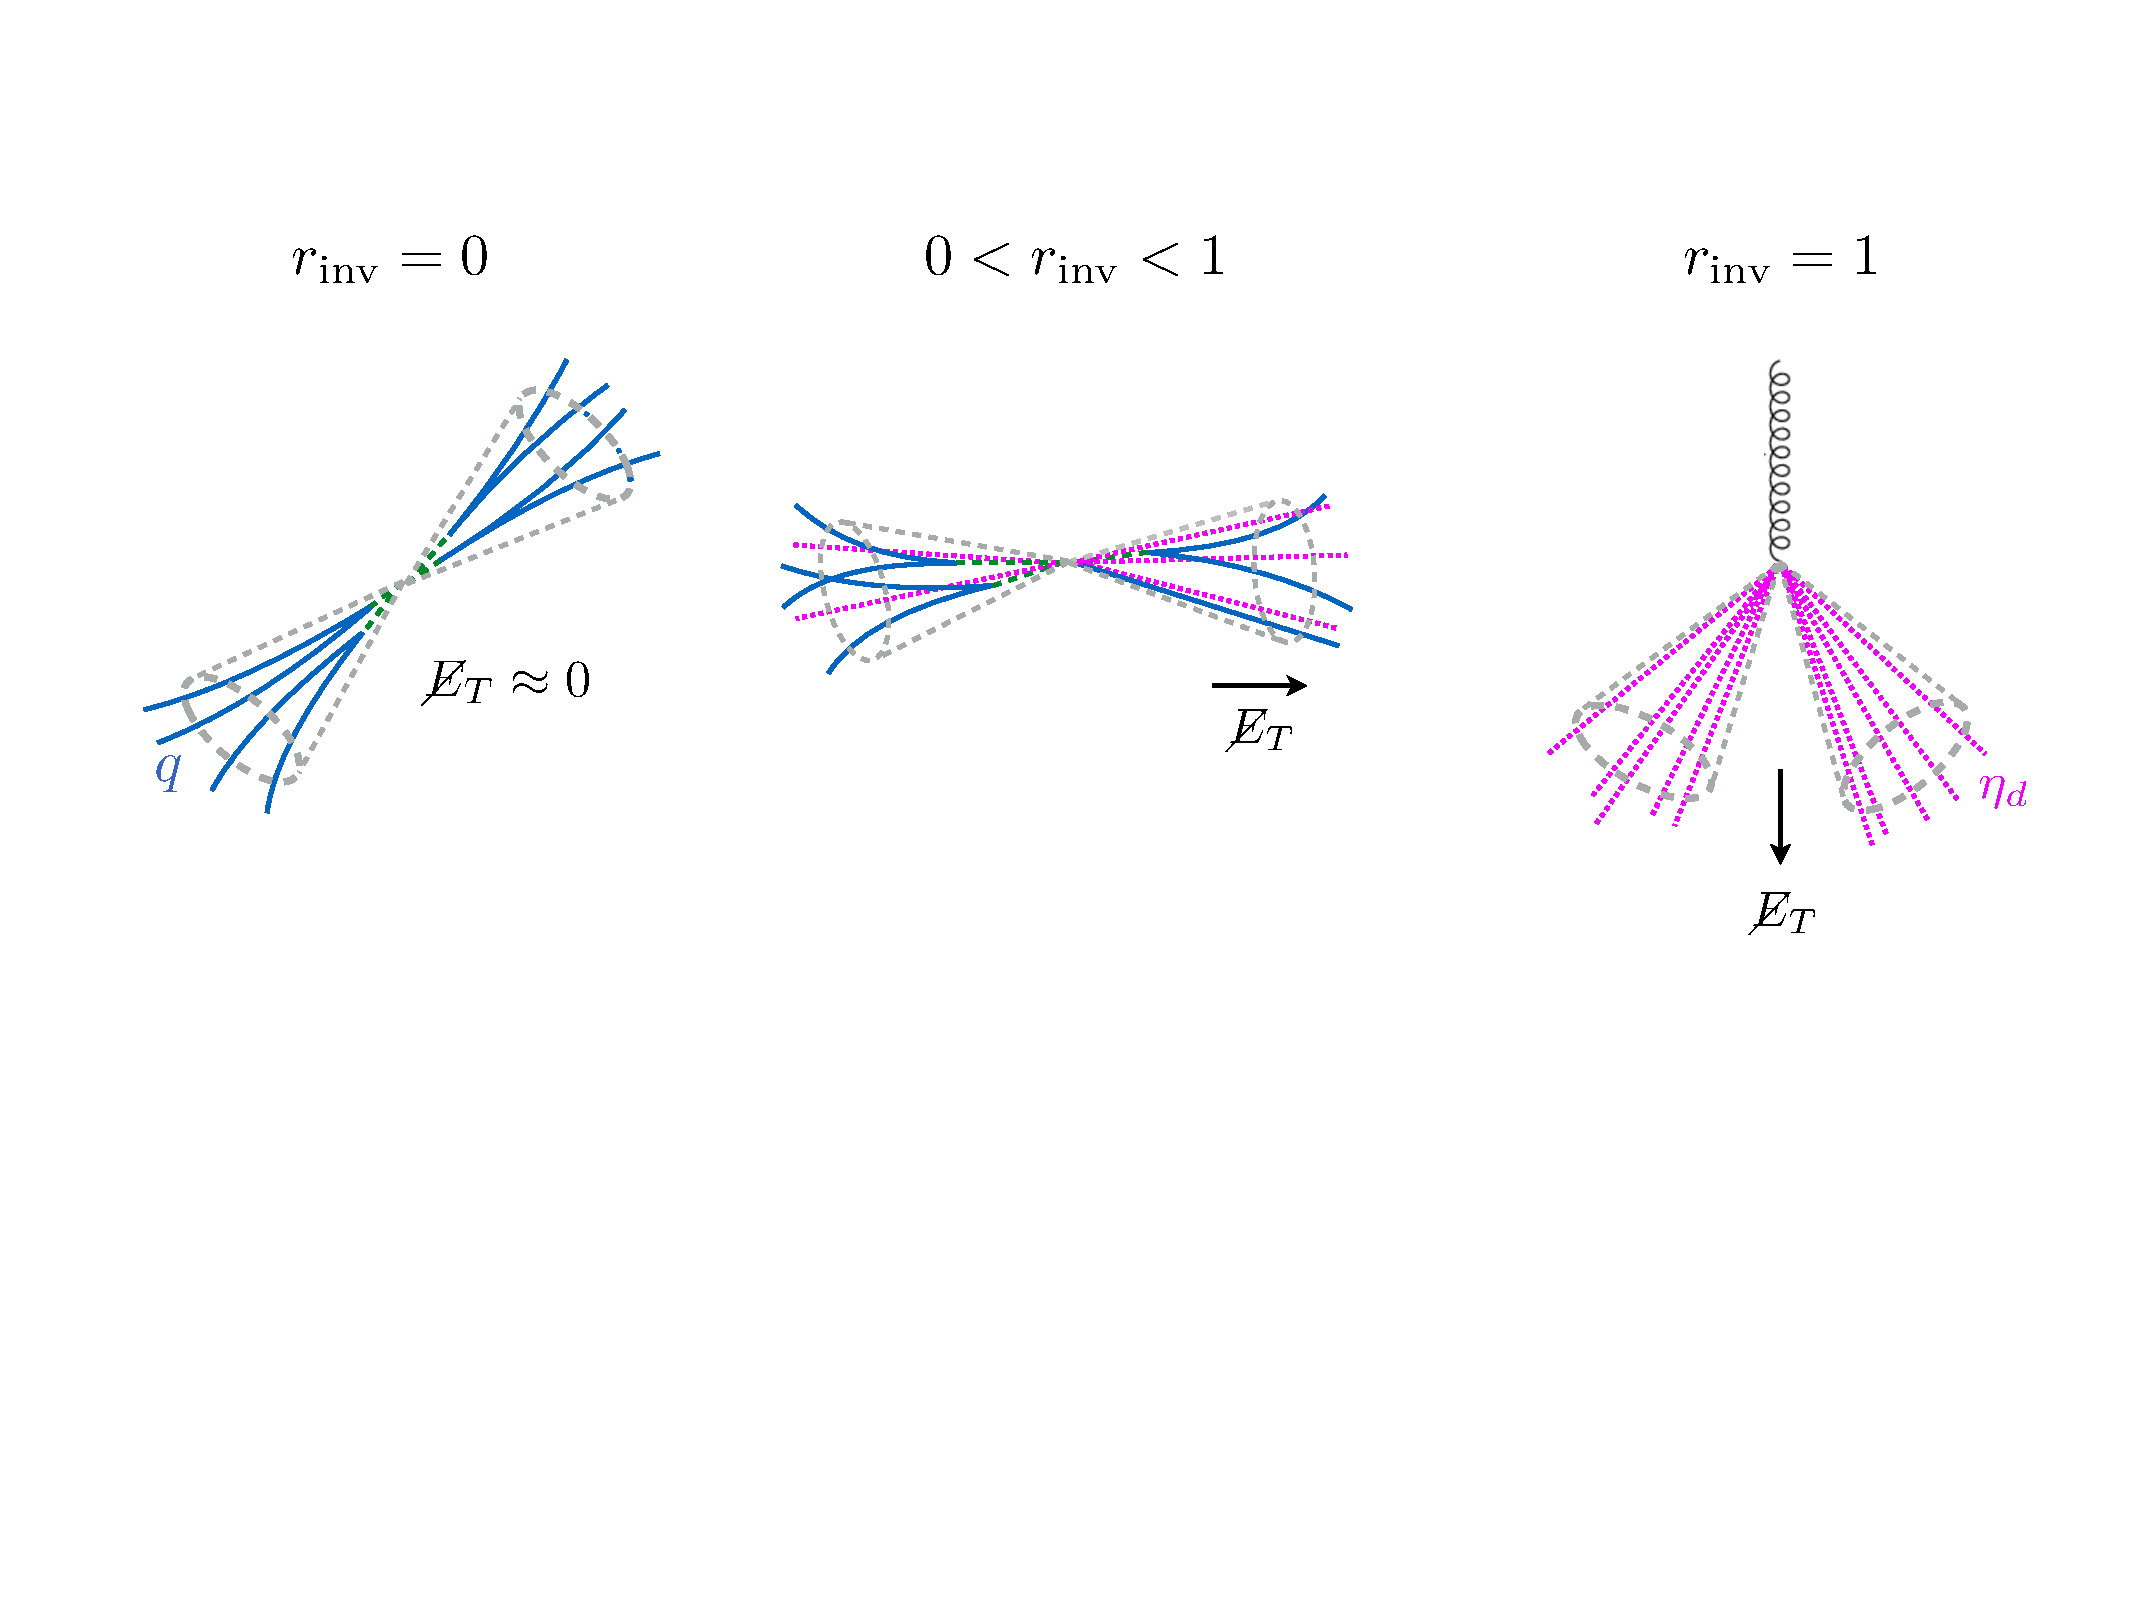
\includegraphics[width=0.85\textwidth]{figures/svj/metfigure.pdf}
\caption[The typical direction of the missing transverse energy relative to the semi-visible jets as a function of the invisible fraction \rinv]{The typical direction of the missing transverse energy \ETslash\xspace (or \ptmiss) relative to the semi-visible jets as a function of their invisible fraction \rinv \cite{Cohen:2017pzm}.}
\label{fig:theory_svj_met_dir}
\end{figure}

\begin{figure}[htbp]
    \centering
    \begin{subfigure}[c]{0.45\textwidth}
    \centering
        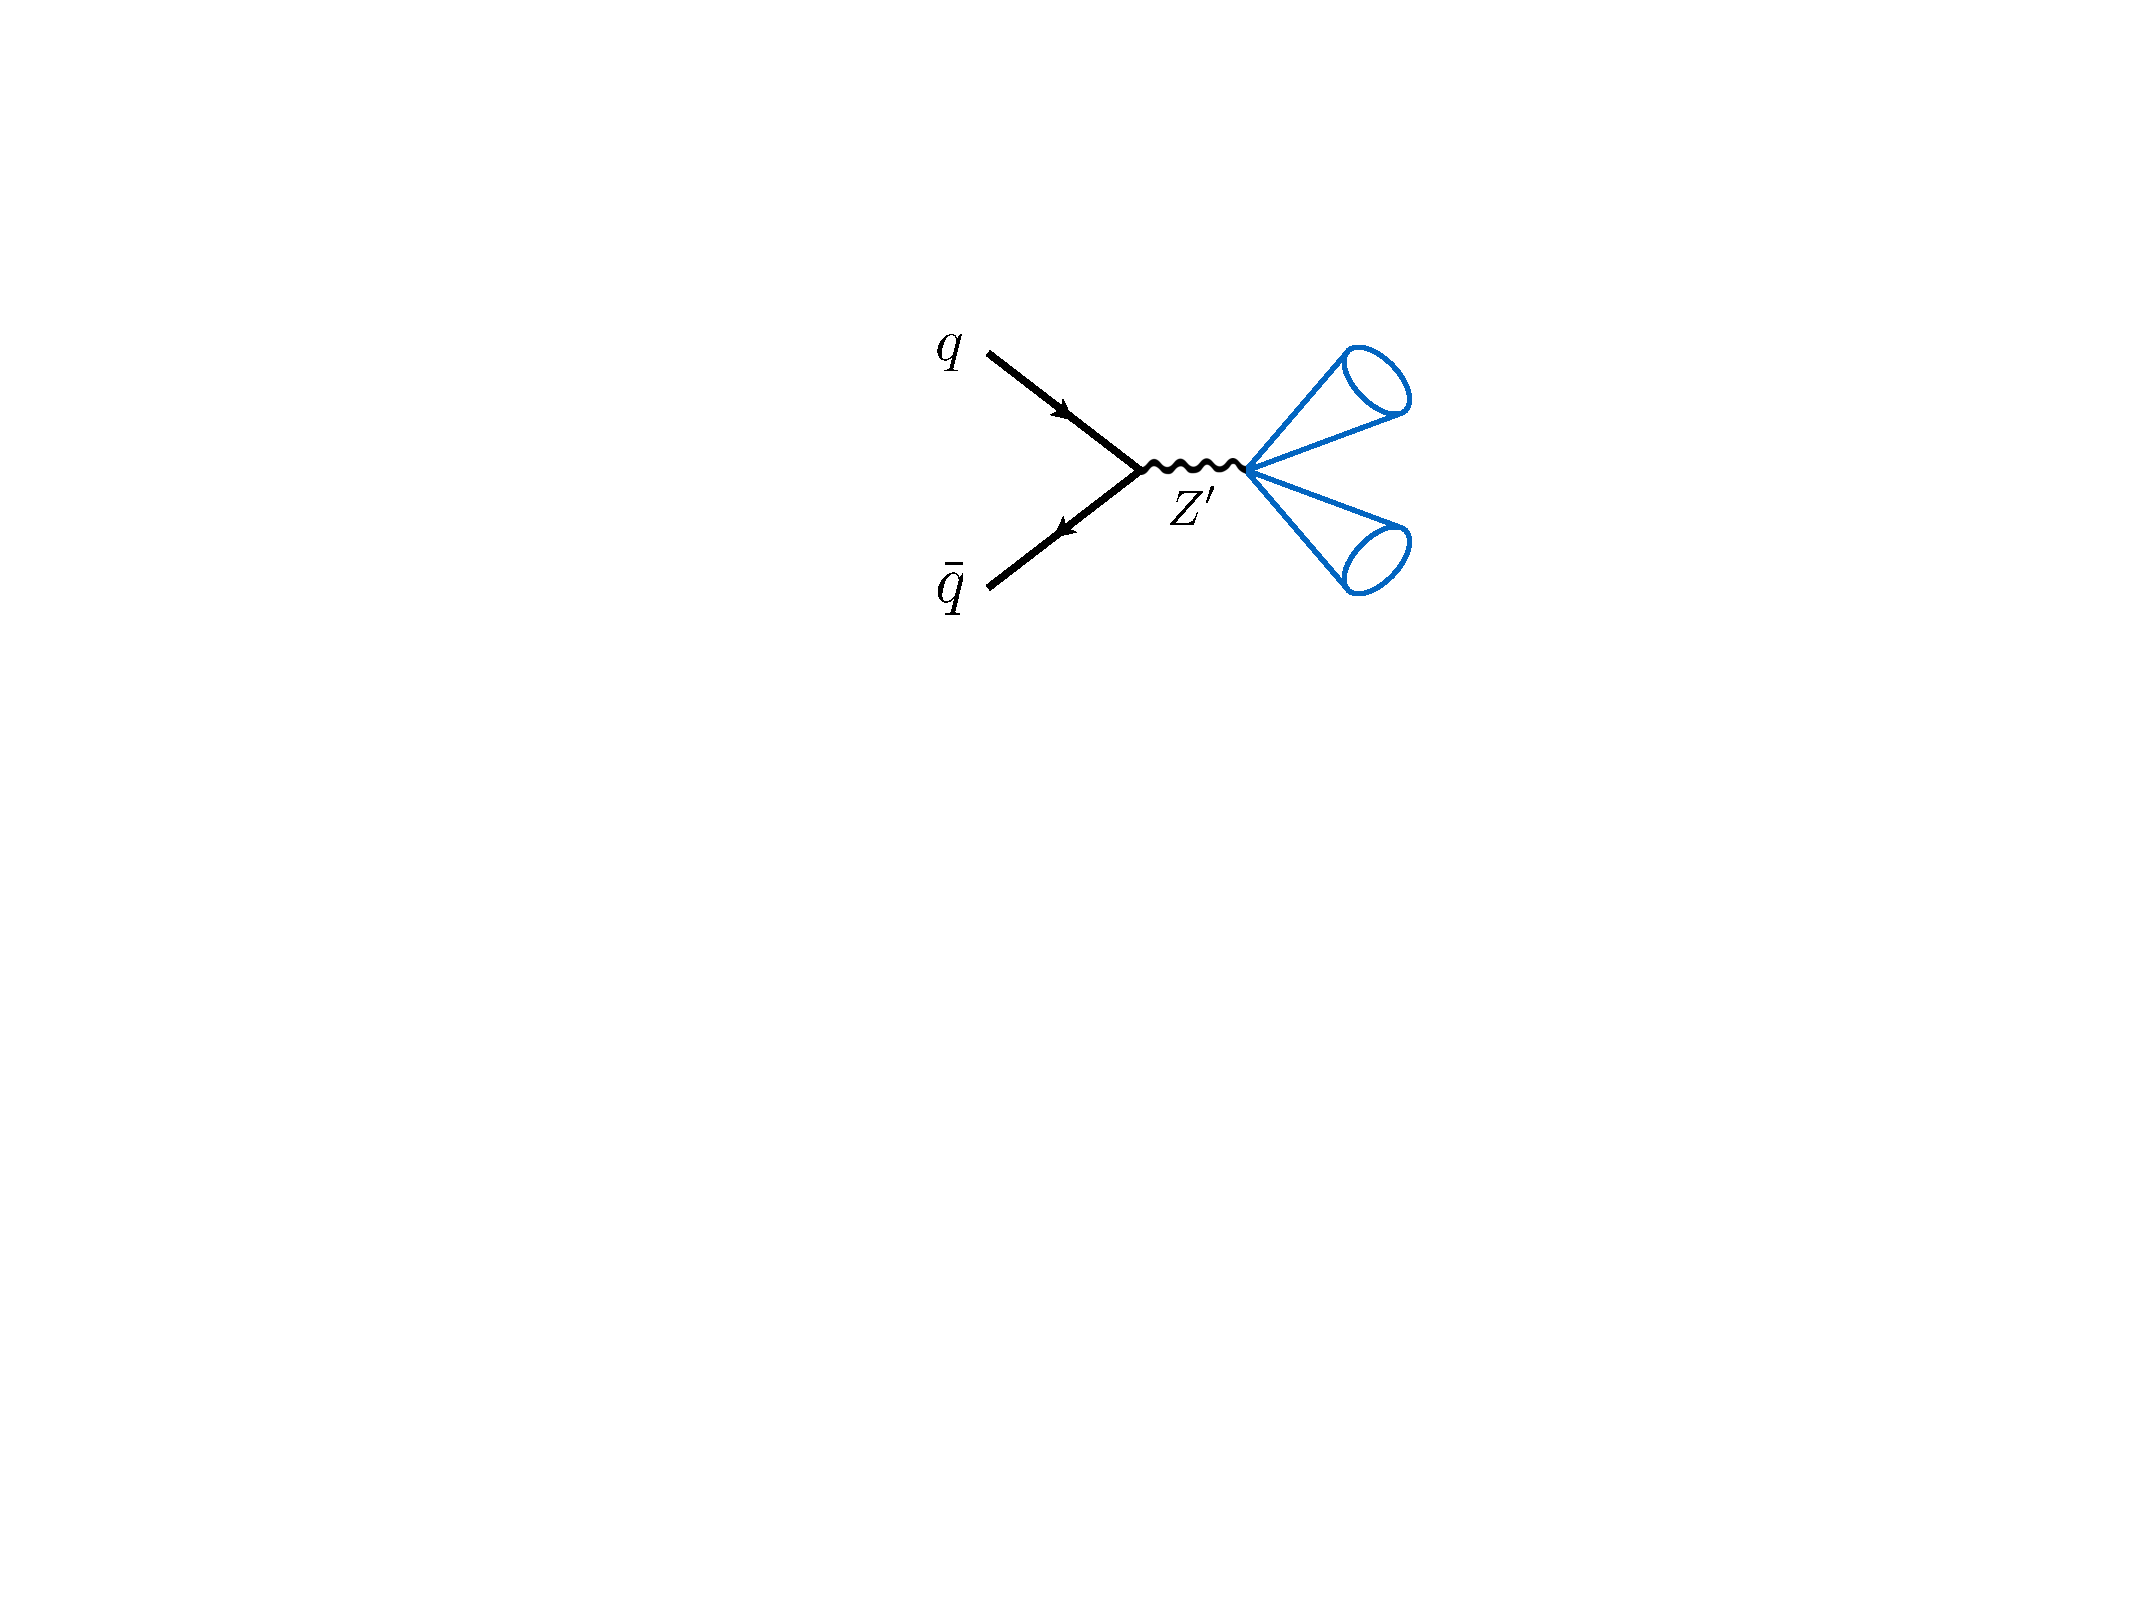
\includegraphics[width=0.7\textwidth]{figures/svj/portals_s.pdf}
        \caption{\schannel}
    \end{subfigure}
    \hfill
    \begin{subfigure}[c]{0.45\textwidth}
    \centering
        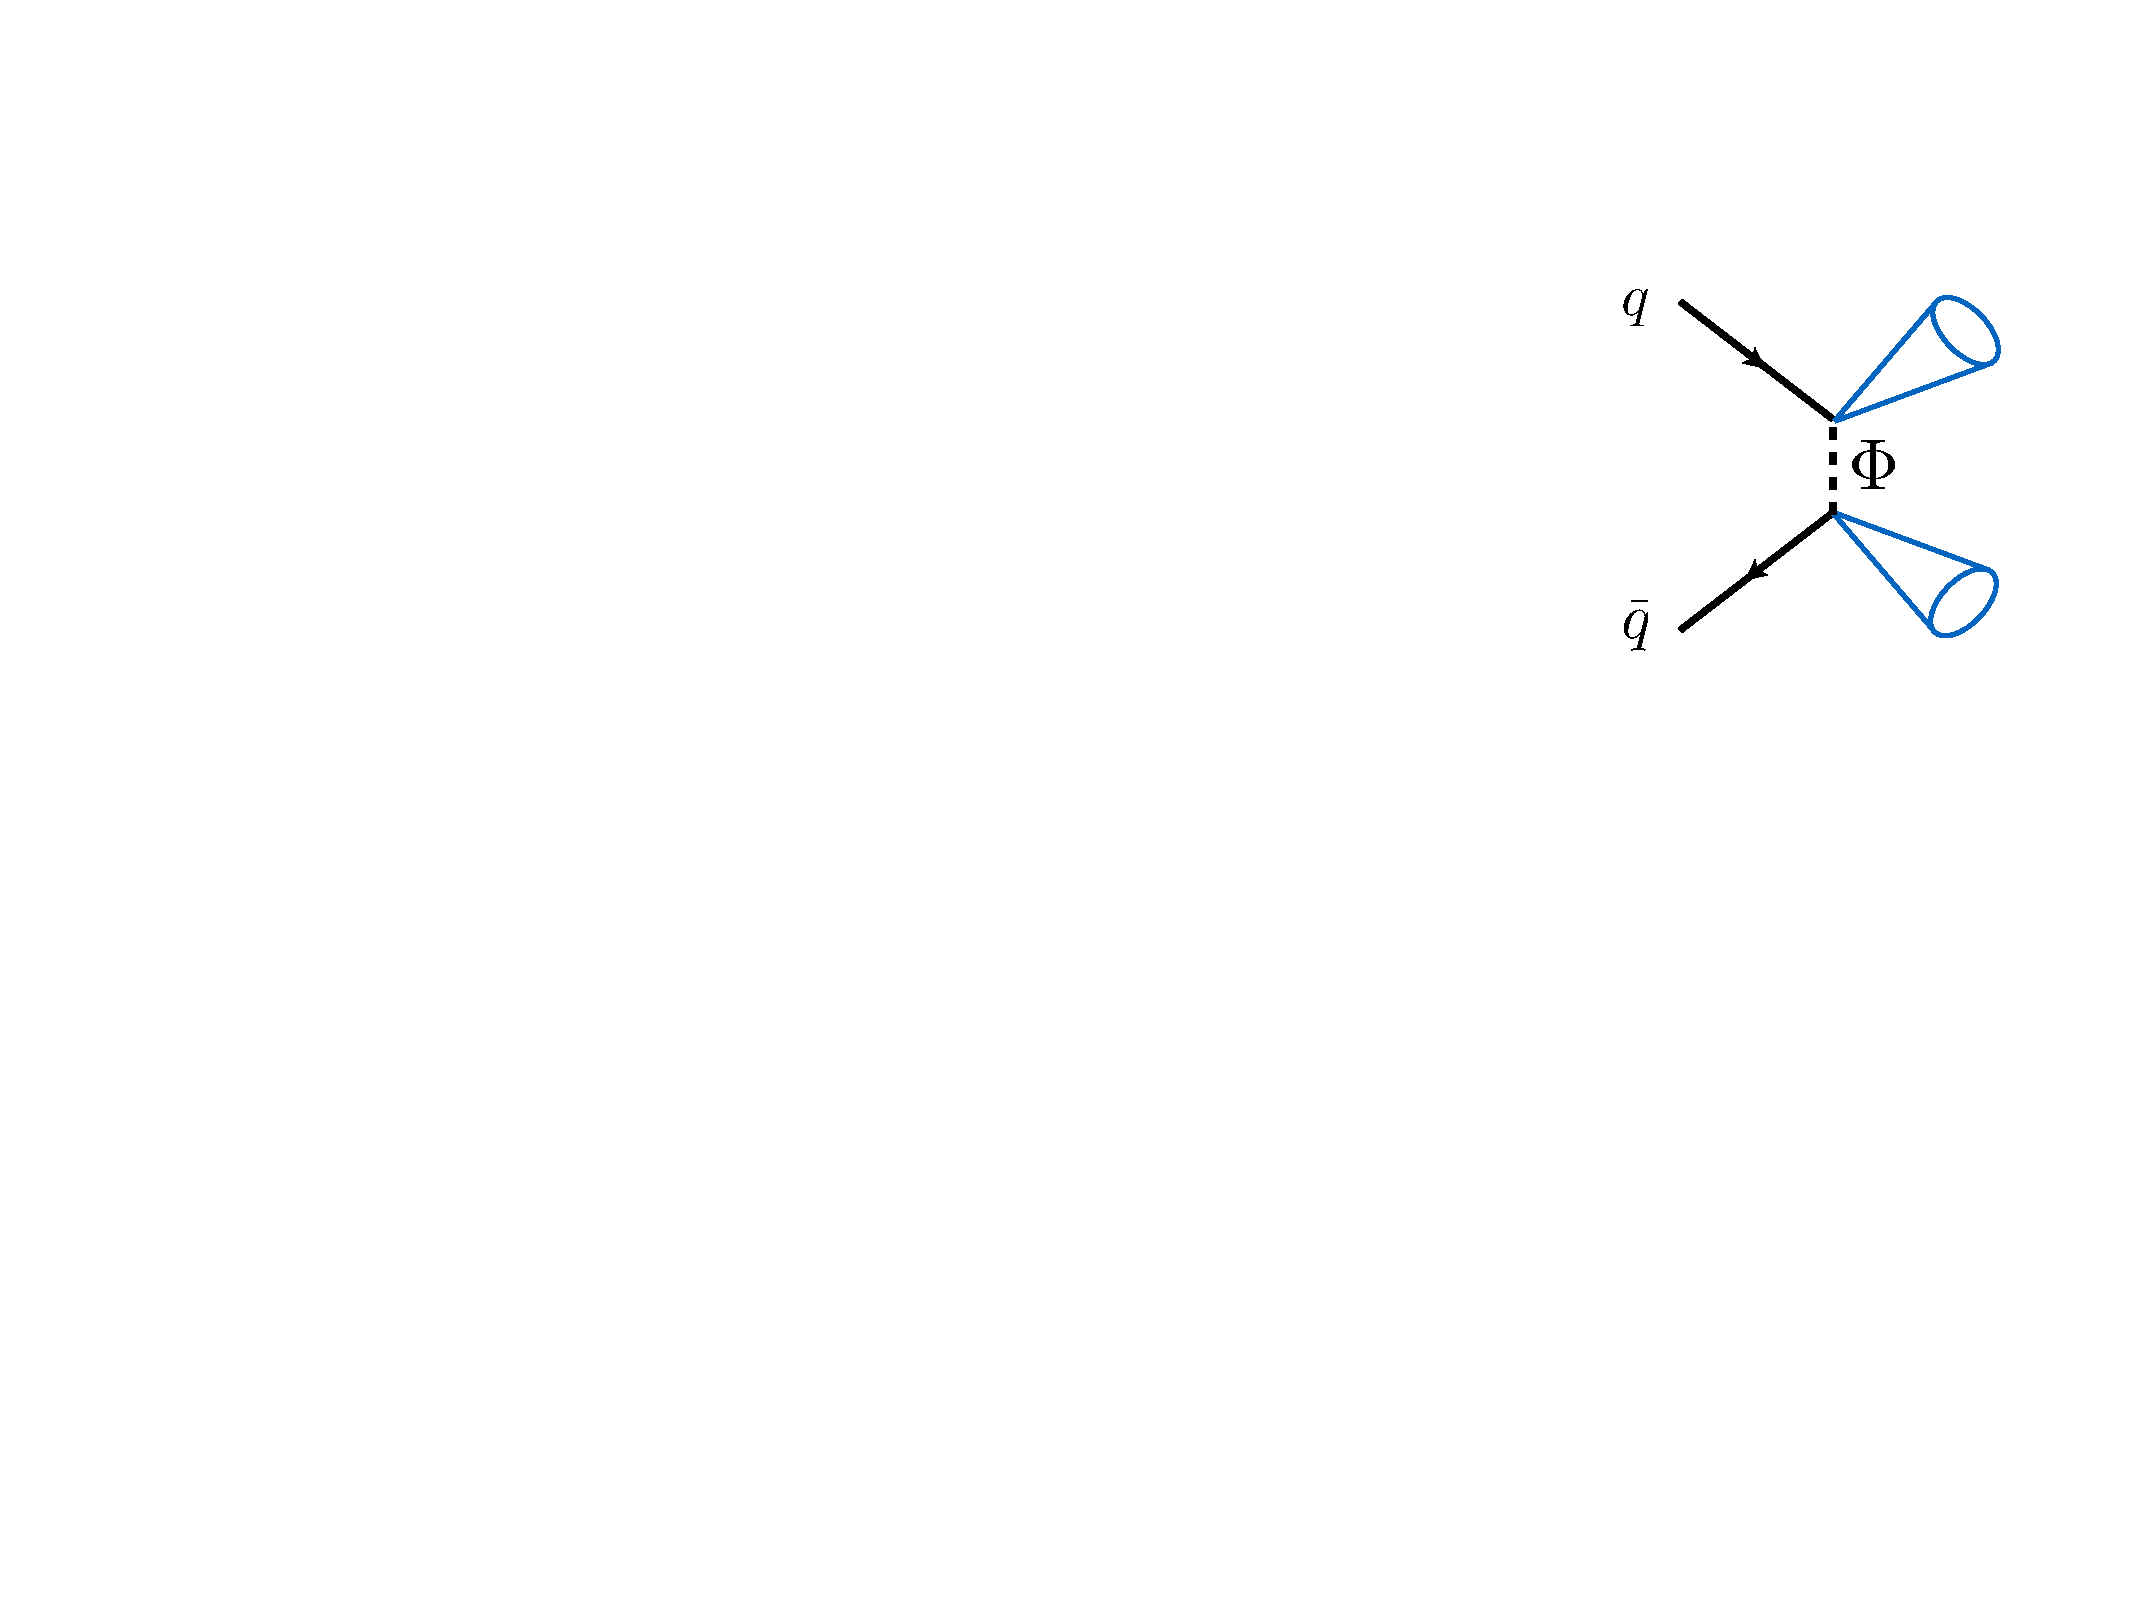
\includegraphics[width=0.7\textwidth]{figures/svj/portals_t.pdf}
        \caption{\tchannel}
    \end{subfigure}
\caption[Example Feynman diagrams for the two main production modes of semi-visible jets. A \PZprime  boson mediates the \schannel process while a bifundamental $\Phi$ mediates the \tchannel process]{Example Feynman diagrams for the two main production modes of semi-visible jets \cite{Cohen:2017pzm}. A \PZprime  boson mediates the \schannel process while a bifundamental $\Phi$ mediates the \tchannel process.}
\label{fig:theory_svj_portals}
\end{figure}

\begin{figure}[htbp]
\centering
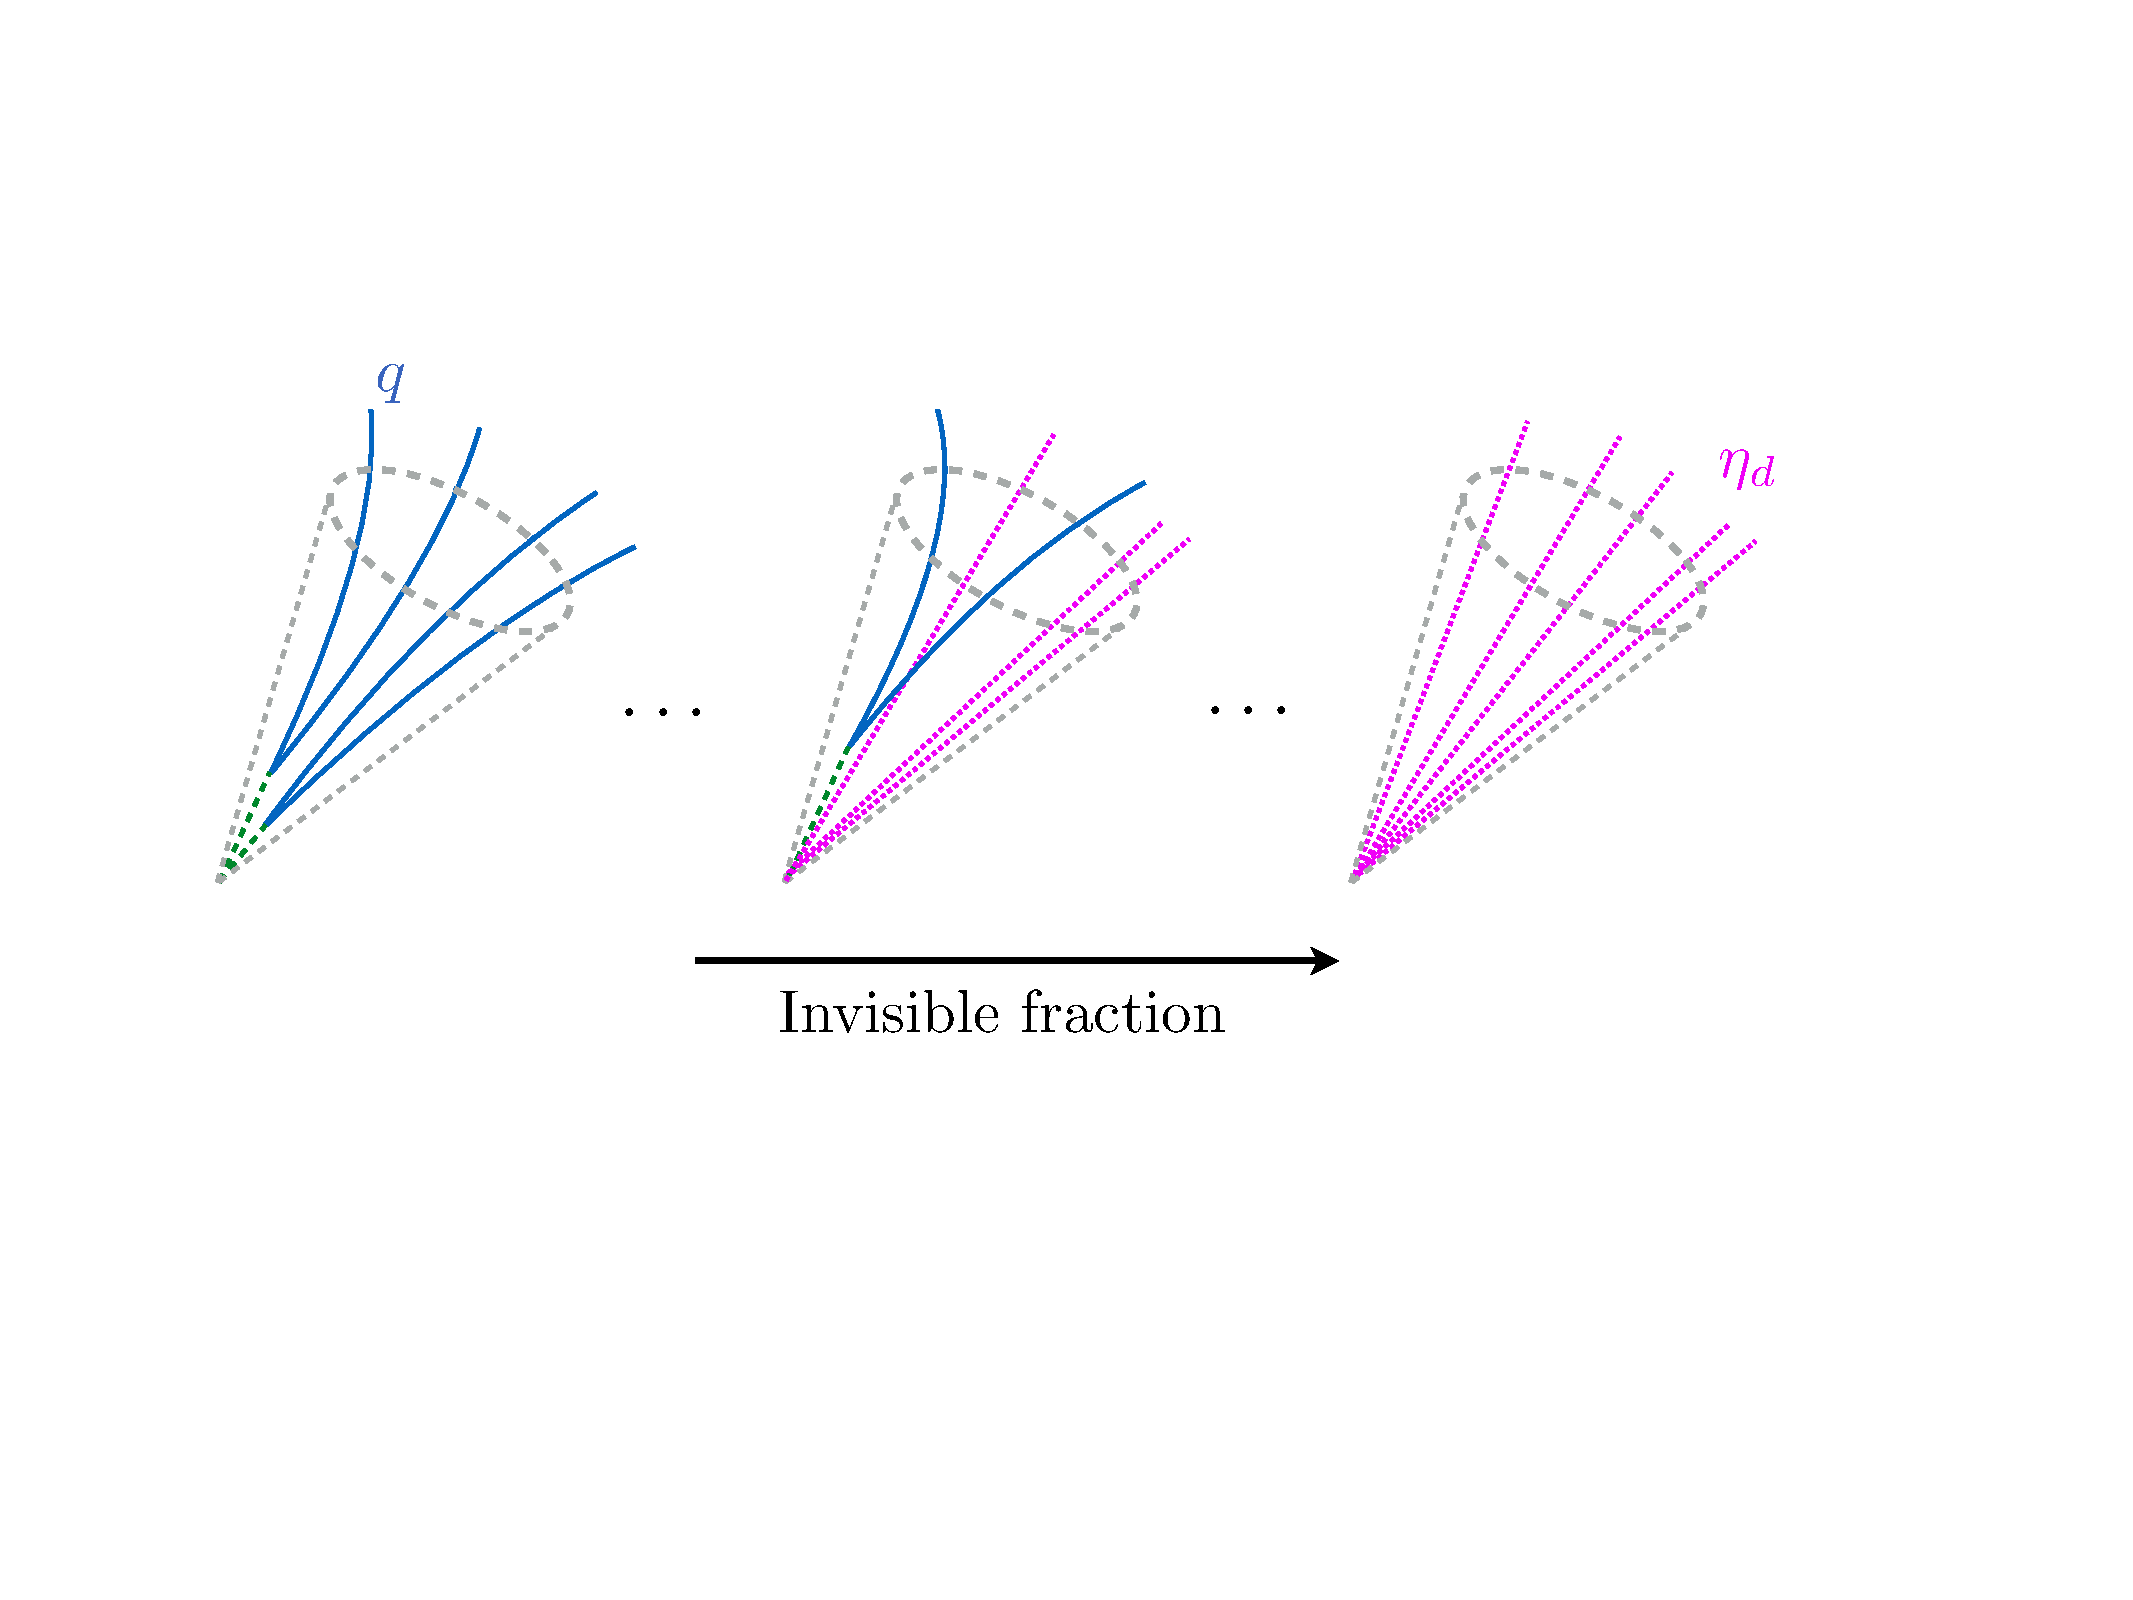
\includegraphics[width=0.75\textwidth]{figures/svj/r_inv.pdf}
\caption[The constituents of a semi-visible jet as a function of its invisible fraction]{The constituents of a semi-visible jet as a function of its invisible fraction \rinv \cite{Cohen:2017pzm}.}
\label{fig:theory_svj_rinv}
\end{figure}
